\usepackage{graphicx} % Required for inserting images
\usepackage{mathtools}
\usepackage[hidelinks]{hyperref}
%\usepackage{bbm}  % for \mathbb and \mathbbm symbols
\usepackage{amsmath,amsfonts,amssymb, amsthm}
\usepackage{cleveref} % this needs to go after hyperref and amsmath

%\usepackage[chapter]{algorithm}  % for algorithm environment, option: use chapters for numering
\usepackage{tikz}
\usetikzlibrary{positioning}

\usepackage{tikz-cd}  % commuting diagrams based on tikz
\usetikzlibrary{calc}
\usepackage{booktabs}  % for clean tables (tabular environment) 
\usepackage{caption}  % for setting caption width
\captionsetup{width=\linewidth}

\definecolor{Green}{rgb}{0, 0.5, 0.2}
\usepackage[dvipsnames]{xcolor}
\usetikzlibrary{decorations.markings}

\usepackage{titlesec}
\titleformat{\chapter}[display]
  {\normalfont\huge\scshape}
  {\thechapter}
  {0.5em}
  {}
  [\vspace{0.5ex}\titlerule]

% Section
\titleformat{\section}
  {\normalfont\Large\scshape}
  {\thesection}
  {0.5em}
  {}

% Subsection
\titleformat{\subsection}
  {\normalfont\large}
  {\thesubsection}
  {0.5em}
  {}

\captionsetup{width=\textwidth, labelfont=bf, font=small}

\definecolor{greenii}{RGB}{20,140,10}
\definecolor{darkgreen}{rgb}{0.00,0.85,0.1}

\newcommand{\red}[1]{{\color{red} {#1}}}
\newcommand{\orange}[1]{{\color{orange} {#1}}}
\newcommand{\blue}[1]{{\color{blue} {#1}}}
\newcommand{\green}[1]{{\color{OliveGreen} {#1}}}

\usepackage[backend=biber, maxbibnames=3,style=alphabetic, backref,backrefstyle=none]{biblatex}
\addbibresource{bachelors.bib}

\AtEveryBibitem{
  \clearfield{issn}
  \clearfield{language}
  \clearfield{note}
  \clearfield{urldate}
}

\AtEveryBibitem{%
  \ifboolexpr{
    ( test {\ifentrytype{article}} or test {\ifentrytype{online}})
    and
    ( not test {\iffieldundef{doi}} or not test {\iffieldundef{eprint}} )
  }
  {\clearfield{url}}
  {}
}

\AtEveryBibitem{%
  \ifboolexpr{
    not test {\iffieldundef{doi}}
    or not test {\iffieldundef{eprint}}
  }
  {\clearfield{url}}
  {}
}

\newcommand{\ket}[1]{\ensuremath{\left| #1 \right\rangle}}
\newcommand{\bra}[1]{\ensuremath{\left\langle #1 \right|}}
\newcommand{\braket}[2]{\ensuremath{\left\langle #1 \middle| #2 \right\rangle}}
\newcommand{\ketbra}[2]{\ensuremath{\left| #1 \right\rangle \left\langle #2 \right|}}
\newcommand{\braopket}[3]{\ensuremath{\left\langle #1 \middle| #2 \middle| #3 \right\rangle}}

\newcommand{\SU}[1]{\mathrm{SU}(#1)}
\newcommand{\SO}[1]{\mathrm{SO}(#1)}
\newcommand{\U}[1]{\mathrm{U}(#1)}
\newcommand{\Sp}[1]{\mathrm{Sp}(#1)}
\newcommand{\GL}[1]{\mathrm{GL}(#1)} % e.g., GL(n, R)
\newcommand{\SL}[2]{\mathrm{SL}(#1, #2)}

\newcommand{\liesl}[1]{\mathfrak{sl}_{#1}} % sl_2 lie algebra.

%\theoremstyle{italics}
\newtheorem{theorem}{Theorem}[section]
\newtheorem{lemma}[theorem]{Lemma}
\newtheorem{fact}[theorem]{Fact}
\newtheorem{conjecture}[theorem]{Conjecture}
\newtheorem{proposition}[theorem]{Proposition}
\newtheorem{corollary}[theorem]{Corollary}
\theoremstyle{definition}
\newtheorem{definition}[theorem]{Definition}
\newtheorem{notation}[theorem]{Notation}
\newtheorem{literature}[theorem]{Literature}
\newtheorem{example}[theorem]{Example}
\newtheorem{assumption}[theorem]{Assumption}
\newtheorem{examples}[theorem]{Examples}
\newtheorem{remark}[theorem]{Remark}
%\newtheorem{proof}{Proof}

\newcommand{\Cat}{\mathbf{Cat}}          % Category of categories
%\newcommand{\VecCat}{\mathbf{Vect}}      % Category of Vector spaces
\newcommand{\Veck}{\mathrm{Vect_k}}
\newcommand{\Rep}{\mathrm{Rep}}          % Representation category
\newcommand{\Hom}{\operatorname{Hom}}    % 
\newcommand{\End}{\operatorname{End}}    % Endomorphism set
\newcommand{\id}{\operatorname{id}}      % Identity morphism
\newcommand{\Hilb}{\operatorname{Hilb_{fd}}}
\newcommand{\del}{\boxtimes}
\newcommand{\sVect}{\mathrm{sVect}}
\newcommand{\gVSpace}[1]{\mathrm{Vec}_{#1}} % Graded Vector Space
\newcommand{\Fib}{\mathrm{Fib}}
\newcommand{\sgotimes}[1]{\otimes_{\scriptscriptstyle#1}} % small Graded Tensor Space
\newcommand{\gotimes}[1]{\otimes_{#1}} % G-graded vectors space 
\newcommand{\ot}{\otimes}
\newcommand{\op}{\oplus}
\newcommand{\bop}{\bigoplus}
\newcommand{\bigot}{\bigotimes}

\newcommand{\Hilbfd}{\mathrm{Hilb_{\text{fd}}}}

\newcommand{\Mod}[1]{\operatorname{Mod}_{#1}}

\newcommand{\FDVec}[1]{\mathrm{FD}#1\mathrm{Vec}}
\newcommand{\VecCat}[1]{\mathrm{Vec}_#1}

\newcommand{\Z}{\mathbb{Z}}
\newcommand{\C}{\mathbb{C}}
\newcommand{\R}{\mathbb{R}}

\newcommand{\CC}{\mathcal{C}}

\newcommand{\ev}{\operatorname{ev}}
\newcommand{\coev}{\operatorname{coev}}

\makeatletter
\definecolor{RoyalBlue}{HTML}{4169E1}
\definecolor{CiteViolet}{HTML}{7B2CBF}
\hypersetup{
    colorlinks=true,
		linkcolor=Maroon,
    %linkcolor = CiteViolet,
		citecolor=RoyalBlue,
    urlcolor=RoyalBlue
}
\makeatother


\definecolor{purple}{rgb}{0.6, 0.1, 0.6}
\definecolor{darkgreen}{rgb}{0.1, 0.5, 0.1}
\definecolor{darkblue}{rgb}{0.1, 0.2, 0.7}

% ==========================================
% Quantum Circuit Macros
% ==========================================

% \drawGate{x}{y}{Label}
\newcommand{\drawGate}[3]{
  \node[draw, fill=white, line width=1pt, minimum width=0.7cm, minimum height=0.7cm] at (#1, #2) {$#3$};
}

% \drawCNOT{x}{y_control}{y_drop}
% Draws a CNOT gate. The target is located at y_control - y_drop.
\newcommand{\drawCNOT}[3]{
  \draw[line width=1pt] (#1, #2) -- (#1, #2 - #3);
  % Control dot
  \filldraw[black] (#1, #2) circle (2.5pt);
  \draw[line width=1pt, fill=white] (#1, #2 - #3) circle (4pt);
  \draw[line width=1pt] (#1-4pt, #2 - #3) -- (#1+4pt, #2 - #3);
  \draw[line width=1pt] (#1, #2 - #3 - 4pt) -- (#1, #2 - #3 + 4pt);
}

% \drawMeasurement{x}{y}
\newcommand{\drawMeasurement}[2]{
  \node[draw, fill=white, line width=1pt, minimum width=0.8cm, minimum height=0.6cm] at (#1, #2) {};
  \draw[line width=0.8pt] (#1-0.25, #2-0.1) arc (180:0:0.25);
  \draw[line width=0.8pt, ->] (#1, #2-0.1) -- (#1+0.2, #2+0.2);
}

% \drawControlledGate{x}{target_y}{Label}{control_y}
\newcommand{\drawControlledGate}[4]{
  \drawGate{#1}{#2}{#3}
}

% ======
% Braid Macros

% \drawInjectionWeave{x}{y}{Label}{a}{b}{c}
\newcommand{\drawInjectionWeave}[6]{
  \node[draw, fill=white, line width=1pt, minimum width=0.7cm, minimum height=0.7cm] at (#1, #2) {$#3$};
}

\usepackage{libertine}
\usepackage[libertine]{newtxmath}

\tikzset{
    fusionarrow/.style={
        postaction={
            decorate,
            decoration={
                markings,
                mark=at position 0.55 with {\arrow[scale=1.0]{Stealth}}
            }
        }
    }
}

% Left-aligned 3-label fusion tree
\newcommand{\FusionTreeThreeLabel}[5]{%
\begin{tikzpicture}[
    x=0.65cm,
    y=0.65cm,
    baseline={(current bounding box.center)}
]
    \coordinate (A) at (0,2);
    \coordinate (B) at (0.8,2);
    \coordinate (C) at (1.6,2);
    \coordinate (D) at (1.2,0.5);

    \coordinate (Vone) at (0.4,1.5);
    \coordinate (Vtwo) at (0.8,1);

    \draw[fusionarrow] (A) -- (Vone);
    \draw[fusionarrow] (B) -- (Vone);
    \draw[fusionarrow] (Vone) -- (Vtwo);
    \draw[fusionarrow] (C) -- (Vtwo);
    \draw[fusionarrow] (Vtwo) -- (D);

    \node[left=1.5pt, font=\scriptsize] at (Vone) {$#5$};

    \node[above, font=\scriptsize] at (A) {$#1$};
    \node[above, font=\scriptsize] at (B) {$#2$};
    \node[above, font=\scriptsize] at (C) {$#3$};
    \node[left, font=\scriptsize] at (D) {$#4$};
\end{tikzpicture}%
}

\newcommand{\BraidOver}[2]{%
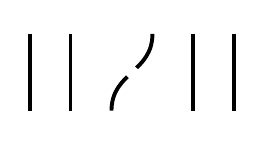
\begin{tikzpicture}[
    x=0.65cm,
    y=0.65cm,
    baseline={(current bounding box.center)}
]
  \draw[line width=1.4] (-2.00, 0.00) to (-2.00, -1.50);
  \draw[line width=1.4] (-1.20, 0.00) to (-1.20, -1.50);
  \draw[line width=1.4] (1.20, 0.00) to (1.20, -1.50);
  \draw[line width=1.4] (2.00, 0.00) to (2.00, -1.50);
  \draw[line width=1.4] (0.40, 0.00) .. controls (0.40, -0.75) and (-0.40, -0.75) .. (-0.40, -1.50);
  \draw[line width=4.5, white] (-0.40, 0.00) .. controls (-0.40, -0.75) and (0.40, -0.75) .. (0.40, -1.50);
\end{tikzpicture}%
}



\newcommand{\FusionTreeThreeLabelRight}[5]{%
\begin{tikzpicture}[
    x=0.65cm,
    y=0.65cm,
    baseline={(current bounding box.center)}
]
    % Incoming leaves
    \coordinate (A) at (1.6,2);
    \coordinate (B) at (0.8,2);
    \coordinate (C) at (0,2);
    \coordinate (D) at (0.4,0.5);

    \coordinate (Vone) at (1.2,1.5);
    \coordinate (Vtwo) at (0.8,1);

    \draw[fusionarrow] (A) -- (Vone);
    \draw[fusionarrow] (B) -- (Vone);
    \draw[fusionarrow] (Vone) -- (Vtwo);
    \draw[fusionarrow] (C) -- (Vtwo);
    \draw[fusionarrow] (Vtwo) -- (D);

    \node[right=1.5pt, font=\scriptsize] at (Vone) {$#5$};

    \node[above, font=\scriptsize] at (A) {$#3$};
    \node[above, font=\scriptsize] at (B) {$#2$};
    \node[above, font=\scriptsize] at (C) {$#1$};
    \node[right, font=\scriptsize] at (D) {$#4$};
\end{tikzpicture}%
}